\section{Auswertung}
\label{sec:Auswertung}
Jegliche Fehlerrechnung wurde mit der python-Bibliothek uncertainties \cite{uncertainties} absolviert.
Trotz dessen sind die Formeln für die Unsicherheiten in den jeweiligen Abschnitten angegeben.
Allgemeine Rechnungen wurden mit der python-Bibliothek numpy \cite{numpy} automatisiert. 
Die graphischen Unterstützungen wurden mit Hilfe der python-Bibliothek matplotlib \cite{matplotlib} erstellt.\\
\subsection{Untersuchung der Filterkurve des Selektiv-Verstärkers}
Die Messwerte zur Untersuchung der Filterkurve sind in der Tabelle \ref{tab:frequence} aufgetragen. 
Diese enthält die gemessene Frequenze und  Ausgangsspannung $U_\text{A}$ und den daraus berechneten Quotienten $\sfrac{U_\text{A}}{U_\text{E}}$, welcher sich aus der
aus der ebend genannten Ausgangsspannung und der konstanten Eingangsspannung $U_\text{E} = \SI{0.01}{\volt}$ zusammensetzt.
\begin{table}
    \centering
    \caption{Gemessene Ausgangsspannung und der daraus berechnete Quotient $\sfrac{U_\text{A}}{U_\text{E}}$ in Abhängigkeit von der Frequenz}
    \label{tab:frequence}
    \begin{tabular} {S[table-format=2.2] S[table-format=1.4] S[table-format=1.2] S[table-format=2.2] S[table-format=1.4] S[table-format=1.2]}
        \toprule
        {$\nu \mathbin{/} \si{\kilo\hertz}$} & {$U_\text{A} \mathbin{/} \si{\volt}$} & {$U$} &
        {$\nu \mathbin{/} \si{\kilo\hertz}$} & {$U_\text{A} \mathbin{/} \si{\volt}$} & {$U$} \\
    \midrule
    20.00 & 0.0085 & 0.85 & 34.60 & 0.0670 & 6.70\\
    21.00 & 0.0095 & 0.95 & 34.61 & 0.0690 & 6.90\\
    22.00 & 0.0003 & 0.03 & 34.62 & 0.0710 & 7.10\\
    23.00 & 0.0004 & 0.04 & 34.63 & 0.0720 & 7.20\\
    24.00 & 0.0006 & 0.06 & 34.64 & 0.0740 & 7.40\\
    25.00 & 0.0007 & 0.07 & 34.65 & 0.0760 & 7.60\\
    26.00 & 0.0010 & 0.10 & 34.66 & 0.0780 & 7.80\\
    27.00 & 0.0030 & 0.30 & 34.67 & 0.0800 & 8.00\\
    28.00 & 0.0160 & 1.60 & 34.70 & 0.0840 & 8.40\\
    29.00 & 0.0210 & 2.10 & 34.75 & 0.0870 & 8.70\\
    30.00 & 0.0280 & 2.80 & 34.77 & 0.0870 & 8.70\\
    31.00 & 0.0390 & 3.90 & 34.80 & 0.0850 & 8.50\\
    32.00 & 0.0565 & 5.65 & 34.81 & 0.0825 & 8.25\\
    33.00 & 0.0940 & 9.40 & 34.82 & 0.0820 & 8.20\\
    34.00 & 0.0220 & 2.20 & 34.83 & 0.0810 & 8.10\\
    34.10 & 0.0190 & 1.90 & 34.84 & 0.0800 & 8.00\\
    34.20 & 0.0230 & 2.30 & 34.85 & 0.0770 & 7.70\\
    34.30 & 0.0290 & 2.90 & 34.86 & 0.0750 & 7.50\\
    34.40 & 0.0380 & 3.80 & 34.87 & 0.0740 & 7.40\\
    34.50 & 0.0500 & 5.00 & 34.88 & 0.0720 & 7.20\\
    34.51 & 0.0510 & 5.10 & 34.89 & 0.0700 & 7.00\\
    34.52 & 0.0530 & 5.30 & 34.90 & 0.0680 & 6.80\\
    34.53 & 0.0540 & 5.40 & 35.00 & 0.0510 & 5.10\\
    34.54 & 0.0560 & 5.60 & 36.00 & 0.0650 & 6.50\\
    34.55 & 0.0580 & 5.80 & 37.00 & 0.0070 & 0.70\\
    34.56 & 0.0590 & 5.90 & 38.00 & 0.0052 & 0.52\\
    34.57 & 0.0610 & 6.10 & 39.00 & 0.0038 & 0.38\\
    34.58 & 0.0630 & 6.30 & 40.00 & 0.0030 & 0.30\\
    34.59 & 0.0650 & 6.50 & { }   & { }    & { } \\
    \bottomrule
\end{tabular}
\end{table}
Mit hilfe der Messwerte lassen sich die Abbildungen \ref{fig:frequence} und \ref{fig:frequencefine} erstellen, welche den gegen die Frequenz
aufgetragenen Spannungsquotienten darstellen.
In der Abbildung \ref{fig:frequence} ist das gesamte gemessene Frequenzspektrum von $\SI{20}{\kilo\hertz}$ bis $\SI{40}{\kilo\hertz}$ aufgetragen.
Jedoch lässt sich dort nicht viel über das Verhalten der Spannung in der Nähe der Resonanzfrequenz erkennen, da nicht nur ein paar Messwerte abweichen, sondern eine
systematische Abweichung vorliegt. Die möglichen Ursachen werden in der Diskussion \ref{sec:Diskussion} näher erläutert.  
Dazu wurde die Abbildung \ref{fig:frequencefine} erstellt, welche den Bereich um  die Resonanzfrequenz besser darstellt und auch einen bessere 
Rekursionskurve ermöglicht.
Die für die Regresson nötige Abbildungsvorschrift ist 
\begin{equation}
    U (\nu) = \frac{c}{\left( \nu^2 - \nu_0^2 \right)^2 + d^2 \nu_0^2} \; \text{.}
\end{equation}
Mittels Regressionsrechnung ergeben sich die Regressionsparameter zu 
\begin{align*}
    \nu_0 & =\num{34.755(2)}       \\
    c     & =\num{3741.23(96067)}  \\
    d     & =\num{0.602(9)}
\end{align*}
Um nun die Güte berechnen zu könne, müssen die Frequenzen $\nu_-$ und $\nu_+$ bei denen die Spannung $U$ den Wert $\sfrac{U_\text{max}}{\sqrt{2}}$ bestimmt werden.
Mittels python lassen sich diese zu
\begin{align*}
    \nu_- &= \SI{34.56}{\kilo\hertz} \\
    \nu_+ &= \SI{34.949}{\kilo\hertz}
\end{align*}
bestimmen, woraus mit Hilfe der Beziehung $REFERENZ$ eine experimentell bestimmte Güte von 
\begin{equation*}
    Q_\text{Exp} = \num{89.508(5)}
\end{equation*}
errechnet werden kann.
\begin{figure}
    \centering
    \caption{Verhältnis der Ausgangs- und Eingangsspannung}
    \label{fig:frequence}
    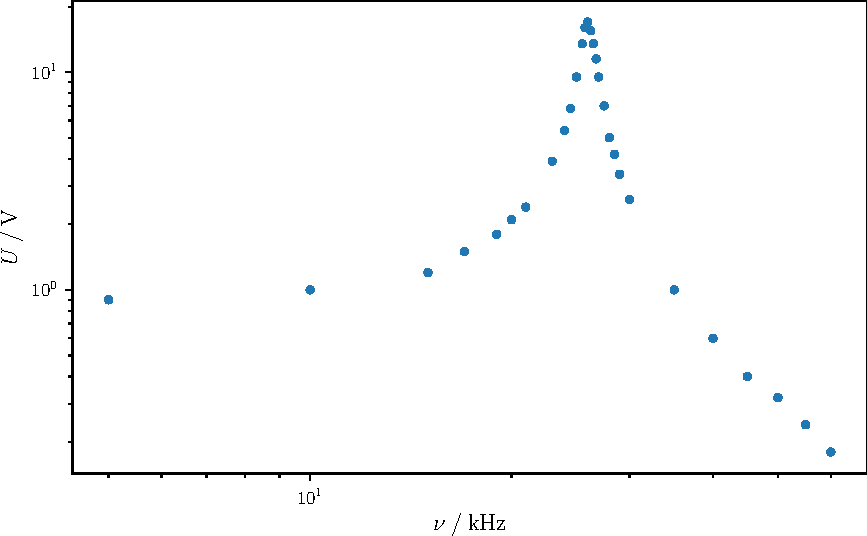
\includegraphics{build/frequence.pdf}
\end{figure}
\begin{figure}
    \centering
    \caption{2.Verhältnis der Ausgangs- und Eingangsspannung im Bereich um die Resonanzfrequenz}
    \label{fig:frequencefine}
    \includegraphics{build/frequencefine.pdf}
\end{figure}
\FloatBarrier
\subsection{Theoretische Bestimmung der Suszeptibilität von $\ce{Dy2O3}$ und $\ce{Nd2O3}$}
Um die Suszeptibilitäten theoretisch bestimmen zu können, müssen zunächst der Spin, der Bahndrehimpuls und der Gesamtdrehimpuls mit Hilfe der Hundschen 
Regeln bestimmt werden.
Mit Hilfe der magnetischen Quantenzahl $m_l$ lässt sich der Gesamtbahndrehimpuls bestimmen, welche von $-l$ bis $l$ geht, wobei l die 
Nebenquantenzahl ist, welche bei der 4f-Schale den Betrag $3$ besitzt. 
Damit der Gesamtbahndrehimpuls maximal ist, trägt diese für alle $m_l$ einen positiven Wert bei. 
Um alle Elektronen zu beschreiben, müssen die größten magnetischen Quantenzahlen wieder abgezogen werden.
Zur Berechnung des Gesamtbahndrehimpulses der 4f-Elektronen von $\ce{Dy2O3}$ wird 
\begin{equation*}
    \lvert L \rvert = \lvert -3 - 2 - 1 + 0 + 1 + 2 + 3 - 3 - 2 \rvert = 5
\end{equation*} 
gerechnet. 
Analog dazu wird der Spin mittels
\begin{equation*}
    S = 7 \cdot \frac{1}{2} - 2  \cdot \frac{1}{2}
\end{equation*}
berechnet. Daraus kann der Gesamtdrehimuls mittels $J = L - s$ errechnet werden.
Nach der Berechnung von $g_J$ lässt sich die Suszeptibilität mit Hilfe der Gleichung \eqref{eqn:chil} errechnen.
Die Momentanzahl pro Volumeneinheit $N$ wird durch
\begin{equation}
    N = 2\cdot\frac{\rho}{M}\cdot N_A 
\end{equation}
bestimmt.
Wobei $N_A$ die Avogadro-Konstante mit $N_A = \SI{6.02214076e23}{\per\mole}$, $M$ die molare Masse und $\rho$ die Dichte der Probe ist. 
Das Borsche Magneton den Wert $\mu_B = \SI{9.2740100783e-24}{\joule\per\tesla}$ und die magnetische Feldkonstante den Wert
$\mu_0 = \SI{1.25663706212e-6}{\newton\per\ampere\squared}$.
Die Boltzmann-Konstante beträgt $k_\text{B} = \SI{1.380649e-23}{\joule\per\kelvin}$.
Als Temperatur wird eine Raumtemperatur von $T = \SI{293.15}{\kelvin}$ angenommen.
Daraus lässt sich die Tabelle \ref{tab:susztheo} erstellen, welche die für die Berechnung der Suszeptibilität nötigen Daten hat.
\begin{table}
    \centering
    \caption{Probenspezfische Daten und die theoretische Suszeptibilität}
    \label{tab:susztheo}
    \begin{tabular} {S[table-format=4.0] S[table-format=1.2]
                     S[table-format=3.3] S[table-format=1.2]
                     S[table-format=1.0] S[table-format=1.0]
                     S[table-format=1.1] S[table-format=1.2]}
        \toprule
        {$\text{Probe}$} & {$\rho \mathbin{/} \si{\gram\centi\metre\tothe{-1}}$} &
        {$M \mathbin{/} \si{\gram\mole\tothe{-3}}$} & {$N \mathbin{/} \SI{e28}{\metre\tothe{-1}}$} &
        {$S$} & {$L$} & 
        {$J$} & {$\chi \cdot \num{e-2}$} \\
    \midrule
    {$\ce{Dy2O3}$} & 7.8  & 372.998 & 2.52 & {$\sfrac{5}{2}$} & 5 & 7.5 & 2.54\\
    {$\ce{Nd2O3}$} & 7.24 & 336.48  & 2.59 & {$\sfrac{3}{2}$} & 6 & 4.5 & 0.25\\
    \bottomrule 
\end{tabular}
\end{table}
\subsection{Experimentelle Bestimmung der Suszeptibilität von $\ce{Dy2O3}$ und $\ce{Nd2O3}$}
\begin{table}
    \centering
    \caption{Gemessene Widerstände und Spannung und die daraus berechnete Widerstandsdifferenz und Suszeptibilität von \ce{Dy2O3}}
    \label{tab:}
    \begin{tabular} {S[table-format=1.1] S[table-format=3.0] S[table-format=1.1] S[table-format=3.0] S[table-format=1.4] S[table-format=0.3]}
        \toprule
        {$U_\text{ohne} \mathbin{/} \si{\milli\volt}$} & {$R_\text{ohne} \mathbin{/} \si{\milli\ohm}$}      &  {$U_\text{mit} \mathbin{/} \si{\milli\volt}$}    &
        {$R_\text{mit} \mathbin{/} \si{\milli\ohm}$}   &  {$\symup{\Delta}R \mathbin{/} \si{\milli\ohm}$}   &  {$\chi \cdot \num{e-3}$}                        \\
    \midrule
    3.5 & 2200 & 7.5 & 565 & 1.635 & 0.644\\
    3.4 & 2200 & 7.5 & 600 & 1.600 & 0.630\\
    3.5 & 2200 & 8.0 & 450 & 1.750 & 0.689\\
    \bottomrule
\end{tabular}
\end{table}